\documentclass[a4paper,12pt]{report}

% Packages et configuration du header
\NeedsTeXFormat{LaTeX2e}
 
%%%%%%%%%%%%%%%%%%%%%%%%%%%%%%%%%%%%%%%%%%%%%%%%%%%%%%%%%%%%%%%%%%%%
%                          P A C K A G E S                         %
%%%%%%%%%%%%%%%%%%%%%%%%%%%%%%%%%%%%%%%%%%%%%%%%%%%%%%%%%%%%%%%%%%%%

\usepackage[french]{babel}
\usepackage{pifont}
\usepackage{lmodern}
\usepackage[T1]{fontenc}
\usepackage[utf8]{inputenc}
\usepackage{lipsum}
\usepackage{amsmath}
\usepackage{amssymb}
\usepackage{mathtools}
\usepackage{graphicx}
\usepackage{xspace}
\usepackage{hyperref}
\usepackage{changepage}
\usepackage[kerning=true]{microtype}
\usepackage{csquotes}
\usepackage{tikzpagenodes}
\usepackage{geometry}
\usepackage{enumitem}
\usepackage{fancyhdr}
\usepackage{calc}
\usepackage{tikz}
\usepackage{adjustbox}
\usepackage{pdfpages}
\usepackage{ragged2e}

\usepackage{paper/imtneStyles/imtnePageDeGarde}
\usepackage{paper/imtneStyles/imtneChapitre}
\usepackage{paper/imtneStyles/imtnePart}


%%%%%%%%%%%%%%%%%%%%%%%%%%%%%%%%%%%%%%%%%%%%%%%%%%%%%%%%%%%%%%%%%%%%%
%                            C O L O R S                            %
%%%%%%%%%%%%%%%%%%%%%%%%%%%%%%%%%%%%%%%%%%%%%%%%%%%%%%%%%%%%%%%%%%%%%

\definecolor{imtneAmbre}{HTML}{fbba00}
\definecolor{imtneAmbreText}{HTML}{f0ab00}
\definecolor{imtneCeleste}{HTML}{00b8de}
\definecolor{imtneCeleste}{HTML}{00b8de}
\definecolor{imtneMarine}{HTML}{001f41}
\definecolor{imtneMarineText}{HTML}{09192b}
\definecolor{imtneGris}{HTML}{eaeaea}
\color{imtneMarineText} % Couleur du texte


%%%%%%%%%%%%%%%%%%%%%%%%%%%%%%%%%%%%%%%%%%%%%%%%%%%%%%%%%%%%%%%%%%%%%
%                          G E O M E T R Y                          %
%%%%%%%%%%%%%%%%%%%%%%%%%%%%%%%%%%%%%%%%%%%%%%%%%%%%%%%%%%%%%%%%%%%%%

\geometry{
  twoside=true,
  head=42.09433pt,
  paperwidth=8.5in,
  paperheight=11in,
  columnsep=2pc,
  top=90pt,
  bottom=65pt,
  inner=50pt,
  outer=50pt,
  marginparwidth=2pc,
  heightrounded
}


%%%%%%%%%%%%%%%%%%%%%%%%%%%%%%%%%%%%%%%%%%%%%%%%%%%%%%%%%%%%%%%%%%%%%
%                     C U S T O M I Z A T I O N                     %
%%%%%%%%%%%%%%%%%%%%%%%%%%%%%%%%%%%%%%%%%%%%%%%%%%%%%%%%%%%%%%%%%%%%%

% Bullet points
\setitemize[1]{label=\textcolor{imtneCeleste}{\ding{228}}}
\setitemize[2]{label=\textbullet}
\setenumerate[1]{font=\bf\color{imtneCeleste}}
\setenumerate[2]{font=\color{imtneMarine}}

% Headers et Footers
\fancyhead[L]{
\includegraphics[width=2cm]{paper/figures/imtne.png}}
% Titre du chapitre en haut à droite setup dans imtnechapitre
\fancyfoot[LO]{\authorShort}
\fancyfoot[LE]{\authorShort}


%%%%%%%%%%%%%%%%%%%%%%%%%%%%%%%%%%%%%%%%%%%%%%%%%%%%%%%%%%%%%%%%%%%%%
%                            M A C R O S                            %
%%%%%%%%%%%%%%%%%%%%%%%%%%%%%%%%%%%%%%%%%%%%%%%%%%%%%%%%%%%%%%%%%%%%%

\def\imtneGetEltSize{%
  \ifdim \paperwidth < \paperheight
    \paperwidth/10
  \else
    \paperheight/10
  \fi%
}

\newcommand{\annote}[3]{{%
  \footnotesize\sffamily%
  \colorbox{#3}{\bfseries\textcolor{white}{#2}}\hspace{-0.3ex}%
  {\color{#3}%
    $\blacktriangleright$%
    \textit{#1}%
    $\blacktriangleleft$%
  }%
}}

\newcommand{\todo}[1]{\annote{#1}{Todo}{imtneAmbreText}}
\newcommand{\td}{\annote{}{}{imtneCeleste}}
\newcommand{\note}[1]{\annote{#1}{Note}{imtneGris}}


\newcommand{\authorShort}{Shaw E.} % Nom de l'auteur raccourci

\begin{document}

\pagenumbering{Roman}
% Page de garde
\imtnepagedegarde
    {Administration système\\\hphantom f \qquad et Intégration continue} % Titre
    {Rapport de stage} % Sous-titre
    {Shaw Eliot} % Nom de l'auteur complet
    {Institut Mines Télécom Nord Europe} % Nom de l'école complète
    {FISE 2025} % Promotion
    {Paul Fush} % Nom du Tuteur de stage
    {Théo Delgutte\\\phantom{lul}\qquad\qquad\qquad \phantom{lul}Rémy Dufrenoy} % Nom du Maître de stage
    {paper/figures/amiralogo.pdf} % Logo entreprise

\cleardoublepage
% Remerciements
\section*{Remerciements}
Je tiens à exprimer ma sincère gratitude envers Katia Hilal et Sébastien Le Gall pour m'avoir offert l'opportunité de travailler dans l'entreprise Amiral Technologies.
C'est grâce à leur générosité et à l'opportunité qu'ils m'ont offerte que j'ai pu intégrer cette entreprise exceptionnelle.

Je souhaite également remercier mon tuteur de stage à l'IMT Nord Europe, Paul Fush, pour son suivi attentif, ses conseils et sa disponibilité.

Je tiens à exprimer ma reconnaissance envers Théo Delgutte, mon maître de stage inital lors de mon arrivée à l'entreprise.
Son accueil a contribué à me permettre de me faire une place au sein de l'équipe d'Amiral Technologies.

Je tiens à exprimer mes sincères remerciements à Rémy Dufrenoy, le maître de stage qui a pris le relais suite au départ de Théo Delgutte.
Son engagement à me transmettre des compétences techniques essentielles et à me guider tout au long de mon stage a été d'une valeur inestimable pour mon développement personnel et professionnel.
En particulier, je suis reconnaissant envers Rémy Dufrenoy pour son généreux soutien alors que j'étais confronté à une situation incertaine.
Son accueil chaleureux, sans préjugés, a eu un impact positif majeur sur mon expérience au sein de l'entreprise.

J'exprime ma gratitude envers l'ensemble de mes collègues au sein d'Amiral Technologies.
Leur soutien amical, leur expertise partagée et leur accueil chaleureux ont grandement facilité mon intégration dans l'entreprise.

Enfin, je tiens à remercier ma famille et mes amis pour leur soutien inconditionnel.
Leur relecture attentive de mon rapport de stage et leur encouragement ont été une source constante de motivation pour moi.

Je tiens à exprimer ma reconnaissance envers toutes les personnes qui ont joué un rôle essentiel dans mon parcours professionnel et personnel durant ce stage.
Vos contributions et votre engagement ont été inestimables, et je suis honoré d'avoir eu l'opportunité de travailler avec vous et d'apprendre de vous.

\clearpage

% Table des matières
\tableofcontents
\clearpage
\pagenumbering{arabic}
% Mots Clés et Abstract
abstract\\


einstein \cite{einstein}

eeeeeeeee
mots cle

% Content
\imtnechapitre{Introduction}
jolie intro qui dit pk je suisentré à amiral et pk il y avait besoin du refacto



\section{Introduction}
Au sein de l'entreprise Amiral Technologies, j'ai effectué mon stage d'une durée de 14 semaines au département de l'Administration Système Informatique.
 Cette startup française se spécialise dans la prédiction de pannes et se positionne comme un dérivé du CNRS.
 Fondée en 2018 par le Dr Mazen Alamir, directeur de recherche au CNRS, et le Dr Katia Hilal, directrice des opérations de l'entreprise, Amiral Technologies s'appuie sur plus de dix années de recherche académique en théorie du contrôle, automatique et en apprentissage automatique pour développer son logiciel phare, DiagFit.

\section{Amiral Technologies, une startup prometteuse}
\subsection{Description de l'entreprise}
Amiral Technologies est une startup spécialisée dans le développement et la vente du logiciel de prédiction de pannes, Diagfit. Elle se dit être une dérivée (spin-off) du CNRS et participe activement à la recherche dans le domaine de la science des données (datascience)

Fondée en 2018, elle compte actuellement 22 employés et cible principalement trois secteurs d'activité : les transports (entreprises ferroviaires et aéronautiques), l'industrie manufacturière (dans le cadre de l'industrie 4.0) et le secteur de l'énergie et du nucléaire.
\newpage
\subsection{Une entreprise dans un marché exigeant}
\subsubsection{Les entreprises clientes}
Reconnu pour la qualité du logiciel Diagfit, plusieurs clients de renom ont fait appel à l’expertise d’Amiral Technologies afin d'améliorer leur programme de maintenance de leurs équipement.

La startup s'oriente vers trois secteurs précis pour canaliser leur méthode de communication : le secteur des transports avec les entreprises ferroviaires et aéronautiques, le secteur manufacturier en aidant le développement d'une industrie 4.0 et le secteur de l'énergie et du nucléaire.

\vspace{10px}
{\begin{minipage}[c]{0.33\textwidth}

\includegraphics[width=0.8\textwidth]{paper/figures/sncf.pdf}
\end{minipage}
\begin{minipage}[c]{0.5\textwidth}

\includegraphics[width=0.8\textwidth]{paper/figures/mersen.pdf}
\end{minipage}

\begin{minipage}[c]{0.5\textwidth}

\includegraphics[width=0.8\textwidth]{paper/figures/thales.pdf}
\end{minipage}
\begin{minipage}[c]{0.5\textwidth}

\includegraphics[width=0.8\textwidth]{paper/figures/airbus.pdf}
\end{minipage}
}Figure
\label{fig:mon_image}

\subsubsection{Le logiciel Diagfit}
Il permet aux équipements industriels de fonctionner sans défaut et sans pannes en anticipant les problèmes potentiels grâce à l'analyse de données de capteurs.

DiagFit utilise des modèles d'apprentissage automatique qui le rendent exploitable par une personne sans connaissance de la réalité physique des capteurs et sans connaissance dans la datascience.
L'un des atouts majeurs de DiagFit est sa capacité à traiter une multitude d'équipements différents de manière polyvalente, ce qui le rend adaptable à diverses industries.
Enfin, le logiciel utilise une méthode d'apprentissage est efficace avec seulement 3h de données de capteurs dans un mode de fonctionnement saint.
Les pannes en industrie étant très couteuses, ne pas avoir à en produire pour l'outil est essentiel pour vendre l'utilisation de Diagfit.

La détection de pannes permet d'entreprendre des maintenances prédictives en fonction des données spécifiques à l'appareil en question et non à une moyenne de la classe de ces appareils.
Cette technologie permet alors de réduire les coûts de maintenance en les consacrant uniquement lorsqu'elles sont nécessaires.

\subsection{Organisation interne}
\subsubsection{Une organisation en synergie pour l'innovation}
L'entreprise est basée en Isère dans la ville de Grenoble et fait remarquer sa présence dans les salons spécialisés de Lyon et Paris.

Voici un aperçu des membres clés de l'administration :
\begin{itemize}
    \item \textbf{Katia Hilal} : Présidente et co-fondatrice de l'entreprise, Katia apporte une expertise essentielle dans la vision stratégique de l'entreprise.
    \item \textbf{Mazen Alamir} : Co-fondateur d'Amiral Technologies et directeur de recherche au CNRS, Mazen est le créateur de l'algorythme derrière Diagfit.
    \item \textbf{Simon Gazikian} : Directeur général, Simon joue un rôle crucial dans le développement des partenariats et dans l'orientation globale d'Amiral Technologies.
    \item \textbf{Sebastien Le Gall} : En tant que directeur technique, Sebastien est responsable de la supervision et du développement de l'aspect technique du logiciel DiagFit et assure également une gestion efficace des opérations quotidiennes de l'entreprise.
\end{itemize}\phantom{vide pour separer}\\

Amiral Technologies est composé de différentes équipes en synergie pour pouvoir imaginer un algorythme, le développer en un logiciel et le vendre à de nombreux clients.

Description des groupes qui composent Amiral Technologies:
\begin{itemize}
    \item \textbf{L'équipe commerciale} : Responsable de l'identification et de l'établissement de partenariats avec les entreprises clientes pour promouvoir et vendre DiagFit.
    \item \textbf{Les data-scientists} : Experts en analyse de données, ils utilisent DiagFit pour interpréter les informations collectées par les capteurs et améliorer les prédictions de pannes.
    \item \textbf{Les développeurs fonctionnel-utilisateurs (front-end)}\todo{renommer} : Chargés de concevoir et de développer l'interface utilisateur intuitive et conviviale de DiagFit.
    \item \textbf{Les développeurs techniques (back-end)}\todo{renommer} : Responsables de la conception et du développement des fonctionnalités principales de DiagFit, en garantissant une performance optimale et une intégration harmonieuse des données.
    \item \textbf{Les administrateurs système} : Gèrent les infrastructures et s'assurent que le logiciel DiagFit fonctionne de manière sécurisée et fiable.
\end{itemize}

% \includegraphics[width=0.9\textwidth]{paper/figures/organigramme.pdf}



\subsubsection{Engagement envers la Responsabilité Sociétale des Entreprises}
Amiral Technologies s'engage dans la Responsabilité Sociétale des Entreprises (RSE) en mettant en place des initiatives pour réduire son impact environnemental.
Cependant, certains choix peuvent être critiqués, notamment en ce qui concerne l'utilisation d'outils numériques de signature électronique qui génèrent une surcharge de stockage, ou l'investigation de l'empreinte carbone de l'entreprise sans exploitation des résultats.
Malgré cela, l'entreprise continue de rechercher des solutions durables pour améliorer sa contribution à la RSE.

La RSE est devenue un sujet crucial dans le monde des affaires, reflétant l'intérêt croissant des entreprises à contribuer positivement à la société et à l'environnement.
Dans la plupart des entreprises, les initiatives mises en œuvre pour répondre aux attentes en matière de RSE ont un fort accent sur le pilier écologique.
Cependant, une approche globale de la RSE nécessite également de considérer les autres piliers du développement durable, à savoir le pilier social et économique.
Des efforts peuvent être renforcés pour promouvoir le bien-être des employés, favoriser l'inclusion et l'équité dans le lieu de travail, ainsi que pour soutenir l'économie locale.

En tant que futur professionnel, il est essentiel d'être conscient de l'importance de la RSE et des trois piliers du développement durable.
C'est en contribuant d'une manière volontaire et naturelle que les entreprises pourront jouer un rôle réel dans la société.



\imtnechapitre{Travaux réalisés}
\subsection*{La Culture de la Collaboration et de la Flexibilité}
\subsubsection{Méthode de Travail}
Amiral Technologies opère selon une approche agile, organisée en cycles de travail appelés sprints, d'une durée de 4 à 6 semaines.

Chaque sprint est composé de plusieurs épics (grandes fonctionnalités) rassemblant des tâches liées à un même thème.
À la clôture d'un sprint, une réunion de rétrospective est organisée pour obtenir des retours sur la période écoulée et évaluer les progrès des projets.
De plus, une activité ludique ou un jeu de société est souvent intégré à la réunion, favorisant ainsi la détente et le renforcement de l'esprit d'équipe au sein du département de développement.

Des réunions trihebdomadaires sont également programmées pour créer des opportunités d'échanger sur les avancées immédiates et de discuter des éventuels obstacles rencontrés par les développeurs.
Ces réunions régulières offrent un contexte propice à la résolution collaborative des problèmes et à la génération d'idées.

\subsubsection{Environnement de Travail}
Les locaux d'Amiral Technologies sont aménagés en un vaste open space comportant une vingtaine de bureaux, ainsi que deux salles de réunion.

Les heures de travail varient en fonction des préférences individuelles, avec un consensus autour d'une arrivée vers 9h30 et d'un départ entre 17h00 et 18h00.

Deux jours de télétravail sont accordés chaque semaine aux employés qui le souhaitent.
Pour ma part, j'optais généralement pour le travail au bureau en effectif réduit.

\newpage
\section{Administration système}
Le pôle administration système joue un rôle essentiel dans le maintien en condition opérationnelle des systèmes informatiques de l'entreprise.
Il est responsable de la gestion des sauvegardes et de la récupération des données, assurant ainsi la disponibilité et l'intégrité des informations cruciales.
De plus, il effectue également l'inventaire des équipements et des logiciels, ce qui permet de maintenir une visibilité précise sur les ressources technologiques de l'entreprise.
Grâce à ces responsabilités, le pôle administration système contribue à assurer la continuité des activités, la sécurité des données et la performance des systèmes, ce qui est essentiel pour la productivité et la réussite globale de l'organisation.

Le pôle d'administrateurs système est composé d'une seule personne, Delgutte Théo.
J'ai eu l'occasion de l'assister dans sa mission continue de maintien en condition opérationnelle de la partie informatique de l'entreprise.

\subsection{Objectifs initiaux}
\subsubsection{Réduction des risques}
L'objectif de mon stage était d'atténuer les divers risques potentiels liés à la cyberattaque et à la perte de données.

Ci-dessous une liste des risques identifiés en amont de mon stage :
\begin{itemize}
    \item \textbf{Vulnérabilités Systèmes}
    \item \textbf{Attaques par Hameçonnage}
    \item \textbf{Perte de Données}
    \item \textbf{Accès Non Autorisés}
    \item \textbf{Malwares et Logiciels Malveillants}
    \item \textbf{Défaillance Matérielle}
    \item \textbf{Fuites d'Informations}
\end{itemize}

\subsubsection{Attraction des clients}
De plus, certains clients travaillant avec des données sensibles et des secrets industriels ont manifesté leur intérêt pour l'utilisation du logiciel DiagFit.
Toutefois, ils ont émis une condition spécifique : \hyperref[iso]{l'obtention de la certification ISO 27001 [1]}.
Cette exigence aurait pu constituer un élément différenciateur et potentiellement plus vendeur pour le logiciel, renforçant ainsi son attrait auprès de clients soucieux de la sécurité de leurs données.

\newpage

\subsection{Missions effectuées}
Dans le cadre de mon stage, j'ai entrepris diverses missions visant à améliorer la fonctionnalité, la stabilité et la gestion globale de notre environnement informatique d'Amiral Technologies.

\subsubsection{Gestion de l'infrastructure et de l'inventaire}
J'ai contribué à l'amélioration de notre infrastructure informatique en mettant en place des actions ciblées pour optimiser son fonctionnement.
Cela incluait notamment la résolution d'un problème lié à notre serveur web qui restreignait les modifications par les collaborateurs.
Pour résoudre ce problème, j'ai configuré un serveur de développement dédié, permettant de tester les changements avant leur application sur le site en production.
J'ai également migré les URL en adaptant la base de données du site via des requêtes SQL.

En parallèle, j'ai supervisé l'inventaire matériel et utilisateurs pour une meilleure gestion des ressources et des droits d'accès.
J'ai veillé à ce que les droits d'accès des utilisateurs soient en conformité avec les politiques de sécurité et proposé la conception d'une base de données d'inventaire pour centraliser et suivre les attributions aux utilisateurs.

Enfin, j'ai travaillé sur l'optimisation du schéma réseau en identifiant et en documentant minutieusement les adresses IP associées à chaque machine et service de l'entreprise.
Le schéma de l'infrastructure de l'entreprise est disponible \hyperref[infra]{en annexe}.

Le fonctionnement des services se faisait sous une structure appelée cluster.
La charge de travail était donnée à deux serveurs "maîtres" qui à leur tour répartissaient les tâches à leurs serveurs "esclaves".
Cette structure est souvent utilisée pour permettre de diviser la charge de travail entre plusieurs serveurs et de ne pas dépendre que d'un seul élément pour le fonctionnement des services.
Un schéma de la structure est disponible \hyperref[balancer]{en annexe également}.

\subsubsection{Approche de la Cybersécurité au Quotidien}
La sécurité informatique étant une priorité chez Amiral Technologies, j'ai contribué à mettre en place une approche pratique pour garantir la protection des systèmes et des données des divers clients.
Pour cela, nous avons initié plusieurs axes d'action.

En premier lieu, j'ai participé à la collecte et à la synthèse de documents clés en lien avec \hyperref[iso]{la norme ISO27001}, ce qui nous a permis d'acquérir une solide compréhension des meilleures pratiques en matière de sécurité.

J'ai également eu l'opportunité de participer à une conférence de la Direction du Renseignement et de la Sécurité de la Défense (DRSD), qui m'a apporté des perspectives concrètes sur les enjeux de cybersécurité et d'espionnage industriel international.

Un aspect clé de notre approche a été l'intégration de l'outil Sophos Zero Trust Network Access (ZTNA), qui répond à nos besoins croissants de protection des données et systèmes.
J'ai ensuite organisé une présentation approfondie de l'outil Sophos ZTNA pour assurer sa compréhension et son utilisation par tous les collaborateurs.

Parallèlement, nous avons renforcé notre surveillance en mettant en place Wazuh.
Cette solution nous a permis d'améliorer la détection des menaces en centralisant la surveillance via un serveur Wazuh Manager et un Wazuh Indexer.
L'installation automatisée des agents Wazuh sur les ordinateurs a assuré une surveillance constante et réactive.

Enfin, pour faciliter la gestion et le partage de connaissances, nous avons créé une documentation interne à l'aide de Docusaurus.
Cette plateforme, hébergée sur un PC réhabilité sous Ubuntu, a été organisée en deux parties : une pour les employés et une pour les administrateurs système, couvrant divers scénarios et procédures liées à notre environnement informatique.

Cette approche holistique de la cybersécurité a permis de renforcer notre positionnement tout en garantissant la stabilité et la performance de notre environnement informatique.

\subsection{Retour et critiques sur le projet}
Après environ un mois et demi de mise en place du projet, nous avons organisé une réunion rétrospective pour évaluer son utilité et son impact.
Il est apparu que malgré nos efforts, le projet a entraîné certaines difficultés pour de nombreux collègues lors de sa mise en œuvre.

\subsubsection{Effets contradictoires sur la sécurité}
Les mesures mises en place n'ont pas toujours contribué de manière significative à la réduction des risques, et dans certains cas, elles ont même posé de nouvelles contraintes aux collaborateurs.
Par exemple, l'utilisation d'outils complexes a parfois créé une dépendance envers une seule personne, en l'occurrence l'administrateur système Théo Delgutte.
Cette situation est devenue problématique lors de ses périodes de congés, entraînant des retards et des perturbations dans les opérations.

\subsubsection{Perte de stabilité}
Un autre défi que nous avons rencontré concerne la stabilité des outils utilisés par les collaborateurs de l'entreprise.
Les modifications apportées en cours de route par le sysadmin ont souvent impacté les ressources et les services, générant ainsi une instabilité préjudiciable au bon fonctionnement quotidien.
Cette instabilité a été particulièrement préoccupante pour les employés travaillant à distance, car elle a rendu difficile voire impossible le travail en télétravail sans préavis.

\subsubsection{Perte de l'autonomie}
La décision de limiter les accès aux ressources a également eu des répercussions négatives sur le fonctionnement général de l'entreprise.
Étant donné que le développement de différentes parties du projet est interconnecté et que la documentation d'une partie peut être utile à un autre groupe de personnes, la limitation des accès a entravé la fluidité de la collaboration.
De plus, en tant qu'entreprise de petite taille, les contraintes imposées par cette limitation d'accès semblaient disproportionnées par rapport à d'autres risques potentiellement plus importants.

\newpage

\subsection{Modification des objectifs}
Cette section aborde les ajustements apportés aux objectifs initiaux, visant à résoudre les problèmes identifiés et à reprendre les points bloquants du projet en main.

\subsubsection{Éducation à la cybersécurité}
Au cœur de la cybersécurité réside une composante essentielle : l'éducation des employés pour réduire les risques potentiels.
Dans cette optique, j'ai joué un rôle clé en sensibilisant l'entreprise à l'importance de la cybersécurité grâce à des présentations hebdomadaires.
Ces sessions ont couvert une variété de sujets visant à renforcer la vigilance et les bonnes pratiques parmi les collaborateurs.

Parmi les thèmes abordés, j'ai présenté un guide appréhensible sur l'hygiène de la cybersécurité.
Cela comprenait des conseils pratiques pour naviguer en toute sécurité en ligne, en mettant l'accent sur la prudence face au public, la reconnaissance des extensions de fichiers, la détection d'URL malveillantes et l'utilisation de bloqueurs de traqueurs pour contrôler les publicités et les cookies.

Une attention particulière a été portée sur l'utilisation de gestionnaires de mots de passe pour renforcer la sécurité des comptes en ligne.
Nous avons également abordé les risques liés aux emails malveillants, aux spams et au phishing, en fournissant des méthodes pour les identifier et les éviter.

Un volet de mon travail a consisté à explorer et utiliser l'outil Gophish pour la création d'une campagne de sensibilisation interne sur le phishing.
J'ai récupéré le code source de sites officiels de Microsoft et Gitlab ainsi que d'emails officiels des mêmes groupes dans le but de montrer comment des attaquants pourraient collecter des informations sensibles.
Par la suite, j'ai conçu un message contenant un lien malicieux pour simuler une campagne de phishing.
On peut voir ci-dessous le sondage que j'ai envoyé aux membres de l'entreprise concernant le lien présent dans mon message qui ne concernaît que les membres de l'entreprise présents dans les locaux au moment de la campagne.

\begin{figure}[ht!]
    \centering
    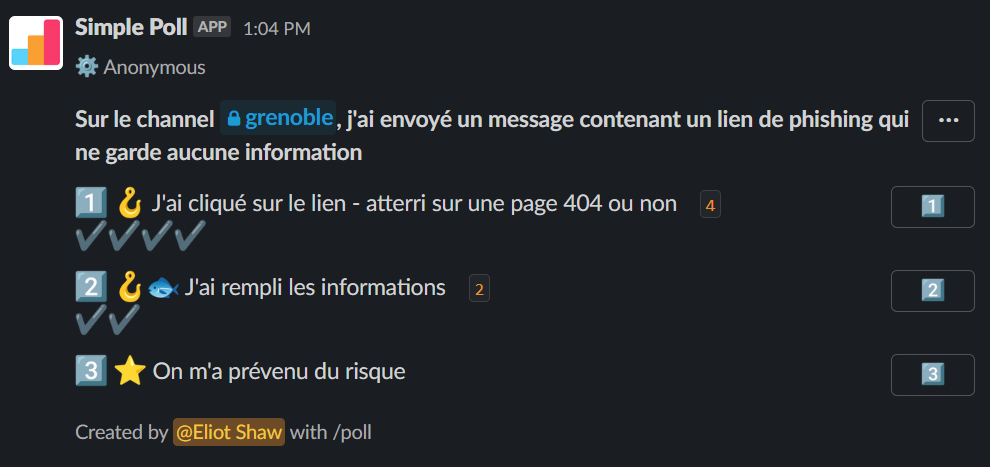
\includegraphics[width=0.66\textwidth]{paper/figures/poll.png}
    \caption{Résultats du sondage concernant le lien de phishing}
    \label{fig:poll}
\end{figure}

Une présentation détaillée a ensuite été faite, montrant les résultats ayant pour objectif de convaincre les employés qu'une attaque informatique peut arriver à tout moment et commettre une imprudence dans le cadre du travail est possible.
Le but de la présentation n'est pas de stigmatiser les personnes s'ayant fait avoir par la campagne mais de permettre aux employés d'aborder le sujet sans tabou pour les habituer à annoncer s'ils ont été victimes d'une attaque.


\subsubsection{Mise en place d'une infrastructure alternative}
Les outils trop complexes à maintenir en condition opérationnelle pour leur coût humain ont été retirés : les agents Wazuh et Sophos ZTNA ont donc été désinstallés pour cette raison.

Un membre de l'entreprise, Rémy Dufrenoy, a également pris de son temps de travail pour créer une nouvelle infrastructure, plus simple pour pouvoir bénéficier d'environnements de travail stables sur lequels ses collègues et lui pourront travailler.

\subsubsection{Modification des droits et autorisations}
Les employés d'Amiral Technologies ont également bénéficié de plus de droits d'accès aux ressources générées par leurs collègues permettant une efficacité de travail plus grande.

En parallèle, un groupe de responsables de l'administration du système fut mis en place pour limiter la création d'un point unique de dépendances.
Une base de données sécurisée de mots de passe contenant les identifiants administrateur pour les ressources fut également créée et partagée entre les responsables.

\subsection{Enseignements appris}
Dans la section qui suit, je partagerai les enseignements que j'ai acquis au cours de cette expérience.

\subsubsection{Shéma des prises de décisions}
Dans ce projet j'ai eu l'occasion d'observer le processus de prises de décisions évolutives.
Le shéma prend en compte le retour d'experience des utilisateurs de l'entreprise pour définir de nouveaux objectifs et diagnostics des besoins.

\begin{figure}[ht!]
    \centering
    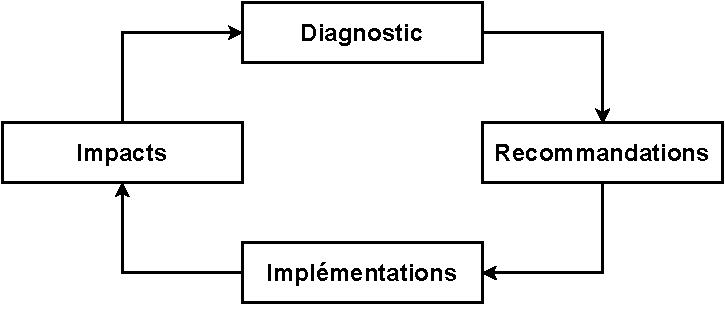
\includegraphics[width=0.5\textwidth]{paper/figures/boucle.pdf}
    \caption{Processus de prise de décisions}
    \label{fig:boucle}
\end{figure}

On peut illuster la première étape du processus décisionnel qui résulte de la craînte de ne pas conquérir de nouvelles parts de marché si les normes de sécurité informatique n'étaient pas obtenues.
\newpage
\begin{figure}[ht!]
    \centering
    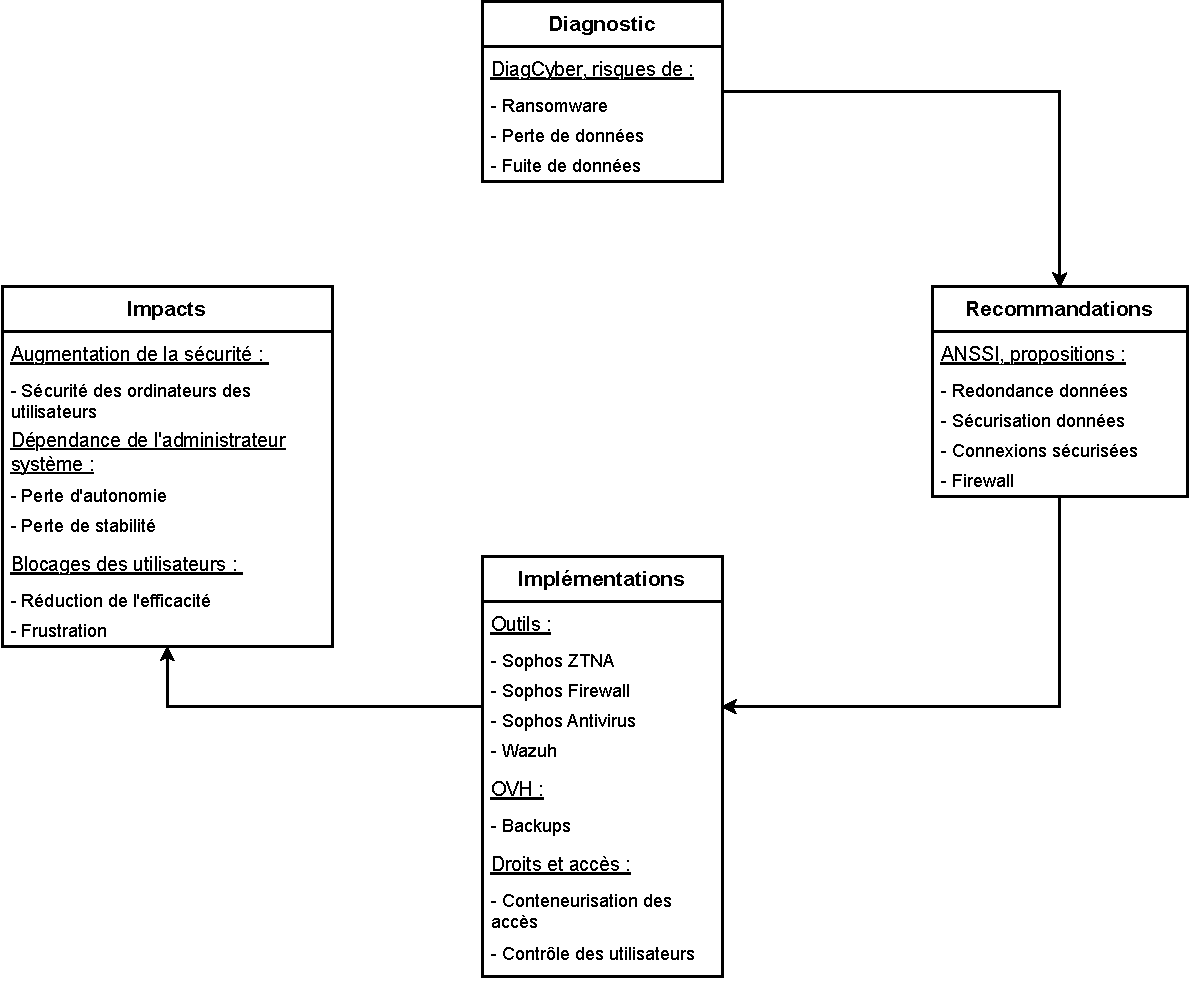
\includegraphics[width=0.75\textwidth]{paper/figures/boucle1.pdf}
    \caption{Première boucle du processus décisionnel}
    \label{fig:boucle1}
\end{figure}

Suite aux retours des employés, nous avons découvert plusieurs points importants non étudiés lors de la pemière observation qui a engendré en une modification des priorités.

\begin{figure}[ht!]
    \centering
    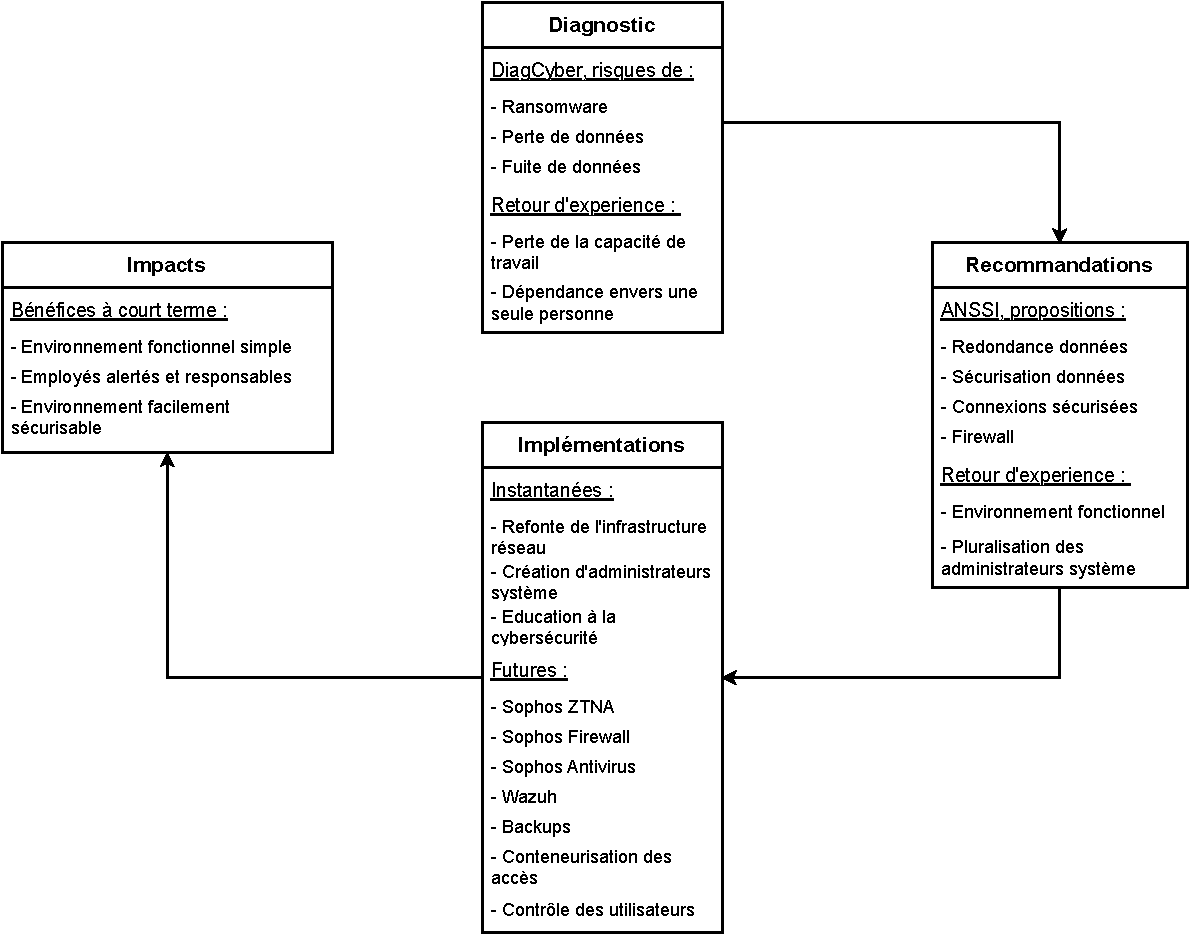
\includegraphics[width=0.75\textwidth]{paper/figures/boucle2.pdf}
    \caption{Seconde boucle du processus décisionnel}
    \label{fig:boucle2}
\end{figure}

\subsubsection{Communication Essentielle}
Lorsque des problèmes ont conduit à des retours en arrière, l'absence de communication adéquate a souvent été à l'origine de ces situations problématiques.
lors de la mise en place de nouvelles restrictions d'accès, les utilisateurs n'ont pas été prévenus des changements à venir.
Cela a provoqué des frustrations et des interruptions dans leur travail quotidien.

Convaincre plutôt qu'imposer est essentiel pour éviter de mécontenter les utilisateurs des services concernés : au lieu d'imposer des nouvelles politiques de sécurité, il serait préférable de présenter les raisons derrière ces changements.

L'importance de l'aspect humain, même dans le domaine de l'administration système, est devenue évidente.
Par exemple, lorsque le système d'exploitation d'un ordinateur ne fonctionnait plus en raison d'un problème matériel, expliquer aux utilisateurs la nature du problème.

Maintenir une communication transparente avec les utilisateurs et expliquer les problèmes rencontrés contribue à renforcer leur confiance et leur satisfaction.

\subsubsection{L'isopérimétrie dans le monde de l'entreprise}
Dans le contexte professionnel actuel, équilibrer l'efficacité au travail et la cybersécurité est crucial.
Les entreprises font face à des menaces de cybersécurité de plus en plus sophistiquées, nécessitant une protection robuste.
Les attaques informatiques évoluent constamment, rendant difficiles la prévention de chaque menace potentielle.

Les administrateurs système jouent un rôle central dans cet équilibre.
Responsables de la sécurité et de la performance des systèmes, ils doivent concevoir des environnements sûrs tout en facilitant la productivité.
Le défi réside dans la recherche du bon équilibre entre des mesures de sécurité strictes et des opérations fluides.

Cela exige des solutions astucieuses de la part des administrateurs système.
L'objectif ultime étant de créer un environnement où la sécurité est maximisée, tout préservant la capacité à livrer de la valeur.






\section{Intégration continue}
\subsection{Technologies utilisées}
\subsubsection{Intégration Continue (CI) avec GitLab}
L'intégration continue (CI) est une pratique de développement logiciel visant à automatiser et à faciliter le processus de construction et de test d'une application.

La construction et le test de Diagfit se fait sur la plate-forme de gestion de développement GitLab avec une série de tâches automatisées, appelées "jobs", qui sont exécutées séquentiellement en réponse aux changements du code source.

\subsubsection{Docker}
Docker est une plate-forme de contenairisation légère qui permet de créer, gérer et exécuter des applications dans des conteneurs.
Les conteneurs Docker encapsulent le code, les bibliothèques et les dépendances d'une application, garantissant une exécution cohérente et prévisible quel que soit l'environnement.
Contrairement aux machines virtuelles traditionnelles, les conteneurs partagent le noyau du système hôte, ce qui les rend plus efficaces en termes de ressources.

L'un des avantages clés de Docker est la portabilité, un seul fichier descriptif appelé dockerfile est respondable pour la création du contenaire.
Grâce à Docker, vous pouvez empaqueter votre application et toutes ses dépendances dans un conteneur unique, puis le déplacer sans effort entre différents environnements, qu'il s'agisse d'un ordinateur portable de développement, d'un serveur de production ou d'un cloud public.

Docker utilise des images pour définir le contenu et la configuration d'un conteneur.
Les images Docker sont des modèles immuables qui contiennent tout ce dont un conteneur a besoin pour s'exécuter.
Quand un fichier décrivant une image est modifié, seule la partie modifiée et ce qui suit est reconstruit, en réutilisant ce qui avait été précédemment construit.

\subsubsection{Docker Compose}
Docker Compose représente un outil simplifiant la gestion d'applications composées de plusieurs conteneurs.
Plutôt que de nécessiter une gestion manuelle de chaque conteneur et de ses paramètres respectifs, Docker Compose offre la possibilité de définir l'ensemble de la configuration d'une application au sein d'un fichier \texttt{docker-compose.yml}.

Dans ce fichier, les services sont spécifiés, lesquels constituent les divers composants de l'application, incluant leurs images Docker, les ports exposés, les variables d'environnement et d'autres options de configuration.
Par la suite, en utilisant la commande \texttt{docker-compose up}, il est possible de lancer simultanément tous les conteneurs, instaurant un environnement cohérent pour l'application.

De plus, Docker Compose simplifie la communication entre les conteneurs d'une application en mettant en place un réseau virtuel par défaut. Ceci permet aux services de se faire référence mutuellement par leur nom de service.


\subsection{Environnement de développement}
\subsubsection{Architecture globale de Diagfit}
Les développeurs travaillaient sur la dernière version en production : Diagfit 2.5.

\todo{mettre drawio archi globale 2.5}

Ci-dessus, l'architecture globale de l'application Diagfit avec tous leur services.
Suite à une refactorisation de l'application, le système s'est grandement simplifié.

\todo{mettre drawio archi globale 2.6}

\subsubsection{Utilisation de Docker et Docker compose}
L'image docker qui était utilisée pour Diagfit lors de la CI demandait une certaine quantité de commandes pour définir l'environnement de l'application.
Reproduire le même environnement pour effectuer des tests était fastidieux et causait des différences entre l'environnement de test en local et celui produit lors de la CI par GitLab.

\subsubsection{Mission confiée}
La mission qui m'a été confiée fut d'optimiser le dockerfile et le fichier Docker Compose utilisés pour le logiciel Diagfit.

J'ai aussi eu l'occasion de créer une image Docker et un fichier Docker Compose pour créer un environnement contrôlé utilisable pour la création du logiciel et également pour les tests des développeurs.

\subsection{Missions effectuées et problèmes rencontrés}
\subsubsection{Optimisation du dockerfile ci et docker compose}
La construction d'une image Docker à partir d'un dockerfile se fait ligne par ligne - étape par étape.
Lors de la reconstruction de l'image, Docker est capable de reprendre la construction au niveau de la première modification dans ce fichier.

L'initialisation de l'environnement de l'image Docker est le téléchargement des packages utilisés pour le logiciel étant long et peu changeant, il etait judicieux de les placer avant la récupération du code en développement.

La réduction des services utilisés nous a également permis de les retirer u fichier docker compose et donc d'accélérer le temps de lancement de l'application.

\subsubsection{Création de multiples Dockerfiles}
La création d'un environnement identique entre la ci de Gitlab et l'ordinateur des développeurs backend était un point important dans la mission qui m'a été proposée.

J'ai pu créer une image spécifique pour le rendu de l'application et une autre pour le développement et les tests unitaires à partir des fichiers existants.

\subsubsection{Modification de l'environnement Gitlab}
Sur la CI de Gitlab, on inclut le fichier dockerfile mais pas l'image construite de l'application.
Il nous a donc fallu lancer une image docker générique pour build l'image docker de développement et de test d'une manière automatisée.

Une des difficultés rencontrées lors de la modification de l'envoironnement Gitlab fut lors de l'implémentation du nouveau job dans la Ci de gitlab : certaines variables fixées au sein du dockerfile ne prenaient pas effet dans le job 


variables gitlab

- des variables ont été set dans l'environnement GitLab en variables globales contenant des informations sensibles

-> on les a enlevées et on a pu utiliser des variables personnalisées pour le programme

\subsubsection{Impacts bénéfiques}
refacto du gitlab-ci
    
- une image à récupérer pour faire les tests, plus besoin de la faire en local

- amélioration de la rapidité d'exectution 12'30" to 11'15" sur le job de test

- Robustesse du docker et de la CI !!!!



\imtnechapitre{Impressions personnelles}
\section{ressenti}
\subsection{changement de maitre de stage}
space : j'ai pas aimé
pas de continuité dans ma mission : cumul de plusieures missions dcp
\subsection{relations humaines}
les potos qui vivent mal leur stage : nofun, suis content de m'en sortir mais SRX ? c dla merde
apprécie les stage dans les petites entreprises, relations humaines
pas de recherche d'optimisation de l'infini, tant mieux
\section{le futuuuur}
\subsection{que faire plus tard ?}
matière : j'hésite encore fort fort entre dev et sysadmin
mon sage de sys s'est trnasformé en stage de dev sans faire expres...
petite entrprise ? ptet pas, mon stage de M1 peut etre un essai pour me faire ma propre idée


\imtnechapitre{Conclusion}
conclu

\cleardoublepage

\imtnechapitre{Annexes et Bibliographie}
\section*{Bibliographie}
\subsubsection{Images utilisées}\label{images}
Les images utilisées sont des ressources qui m'ont été fournies par des employés au sein de l'entreprise ou des diagrammes que j'ai confectionnné lors de mon stage en entreprise.

\subsubsection{ISO/IEC 27001-2022}\label{iso}
Systèmes de management de la sécurité de l'information - Exigences\par
Édition en vigueur : ISO/IEC 27001:2022\par
État actuel : Publiée (stade 60.60)\par
Auteur : 
\begin{itemize}
    \item International Organization for Standardization (ISO)
    \item International Electrotechnical Commission (IEC)
\end{itemize}\par
Date de publication : 2022-10\par
Sources : 
\begin{enumerate}
    \item \href{https://www.cssia.org/wp-content/uploads/2020/01/ISO_27001_Standard.pdf}{\textcolor{imtneCeleste}{Liste de vérification des exigences de la norme ISO 27001 - [Lien vers le PDF]}}
    \item \href{http://www.itref.ir/uploads/editor/2ef522.pdf}{\textcolor{imtneCeleste}{Description détaillée des éléments de la norme ISO 27001 - [Lien vers le PDF]}}
\end{enumerate}

\subsubsection{Définition de la RSE}\label{rse}
Responsabilité sociale des entreprises: une nouvelle stratégie de l'UE\par
Édition en vigueur : 52011DC0681\par
État actuel : Publiée\par
Auteur : 
\begin{itemize}
    \item Commission au parlement européen
    \item Commission au conseil européen
    \item Commission au comité économique européen
    \item Commission au comité social européen
    \item Commission au comité des régions européennes
\end{itemize}\par
Date de publication : 2011\par
Sources : 
\begin{enumerate}
    \item \href{https://www.economie.gouv.fr/entreprises/responsabilite-societale-entreprises-rse}{\textcolor{imtneCeleste}{Site du gouvernemant définissant la RSE - [Lien vers le site]}}
    \item \href{https://eur-lex.europa.eu/legal-content/FR/TXT/?uri=celex:52011DC0681}{\textcolor{imtneCeleste}{Communication de la commission au parlement européen au sujet de la RSE - [Lien vers le site]}}
\end{enumerate}




\newpage
\section*{Annexes}
\subsection*{Infrastructure de l'entreprise}
\begin{figure}[ht!]
    \centering
    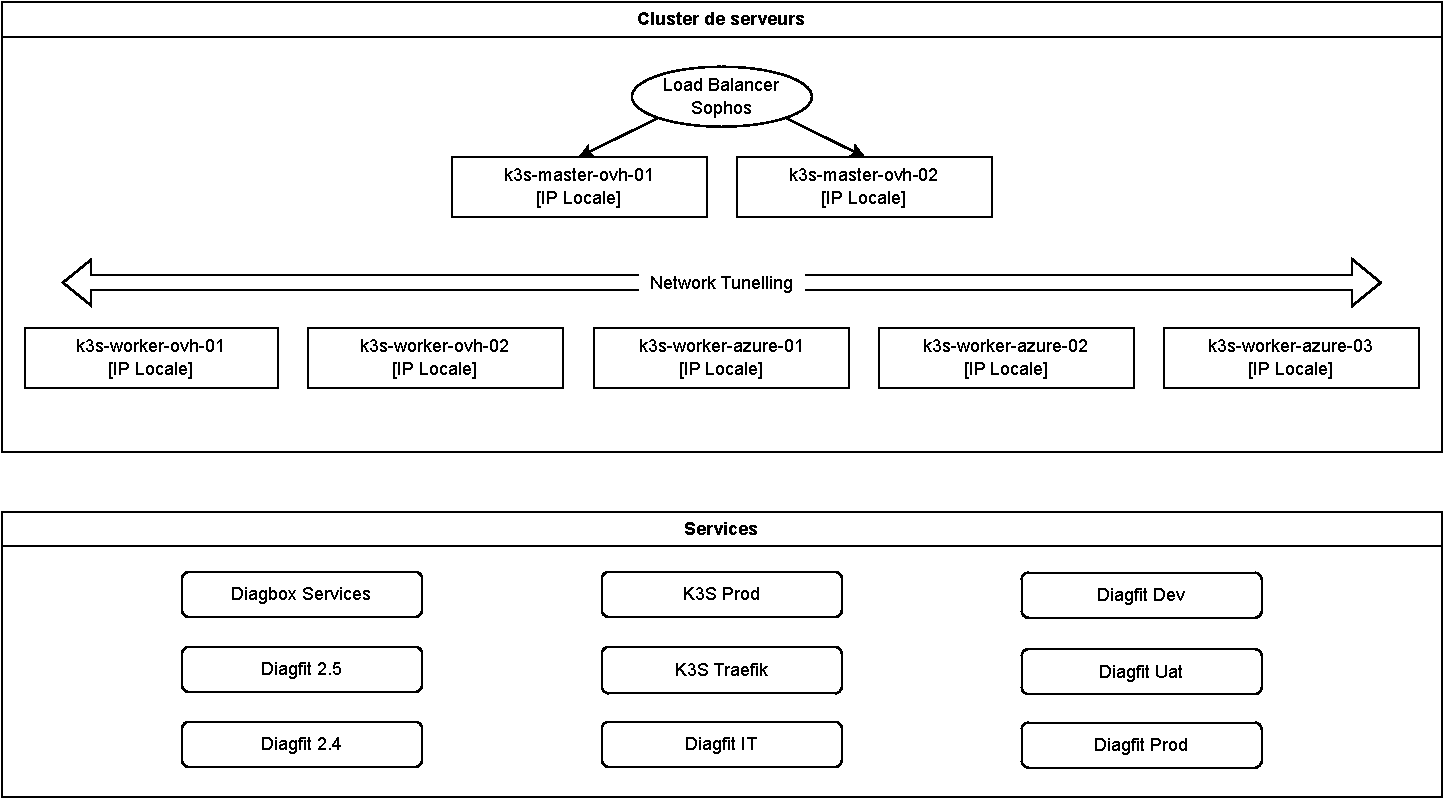
\includegraphics[width=\textwidth]{paper/figures/balancer.pdf}
    \label{balancer}
    \caption{Répartission de la charge de travail entre les différents serveurs}
\end{figure}

\clearpage
\newgeometry{top=0pt, bottom=0pt, inner=0pt, outer=0pt}
\thispagestyle{empty} % Pas de header, footer ou numéro de page
\begin{figure}[ht!]
    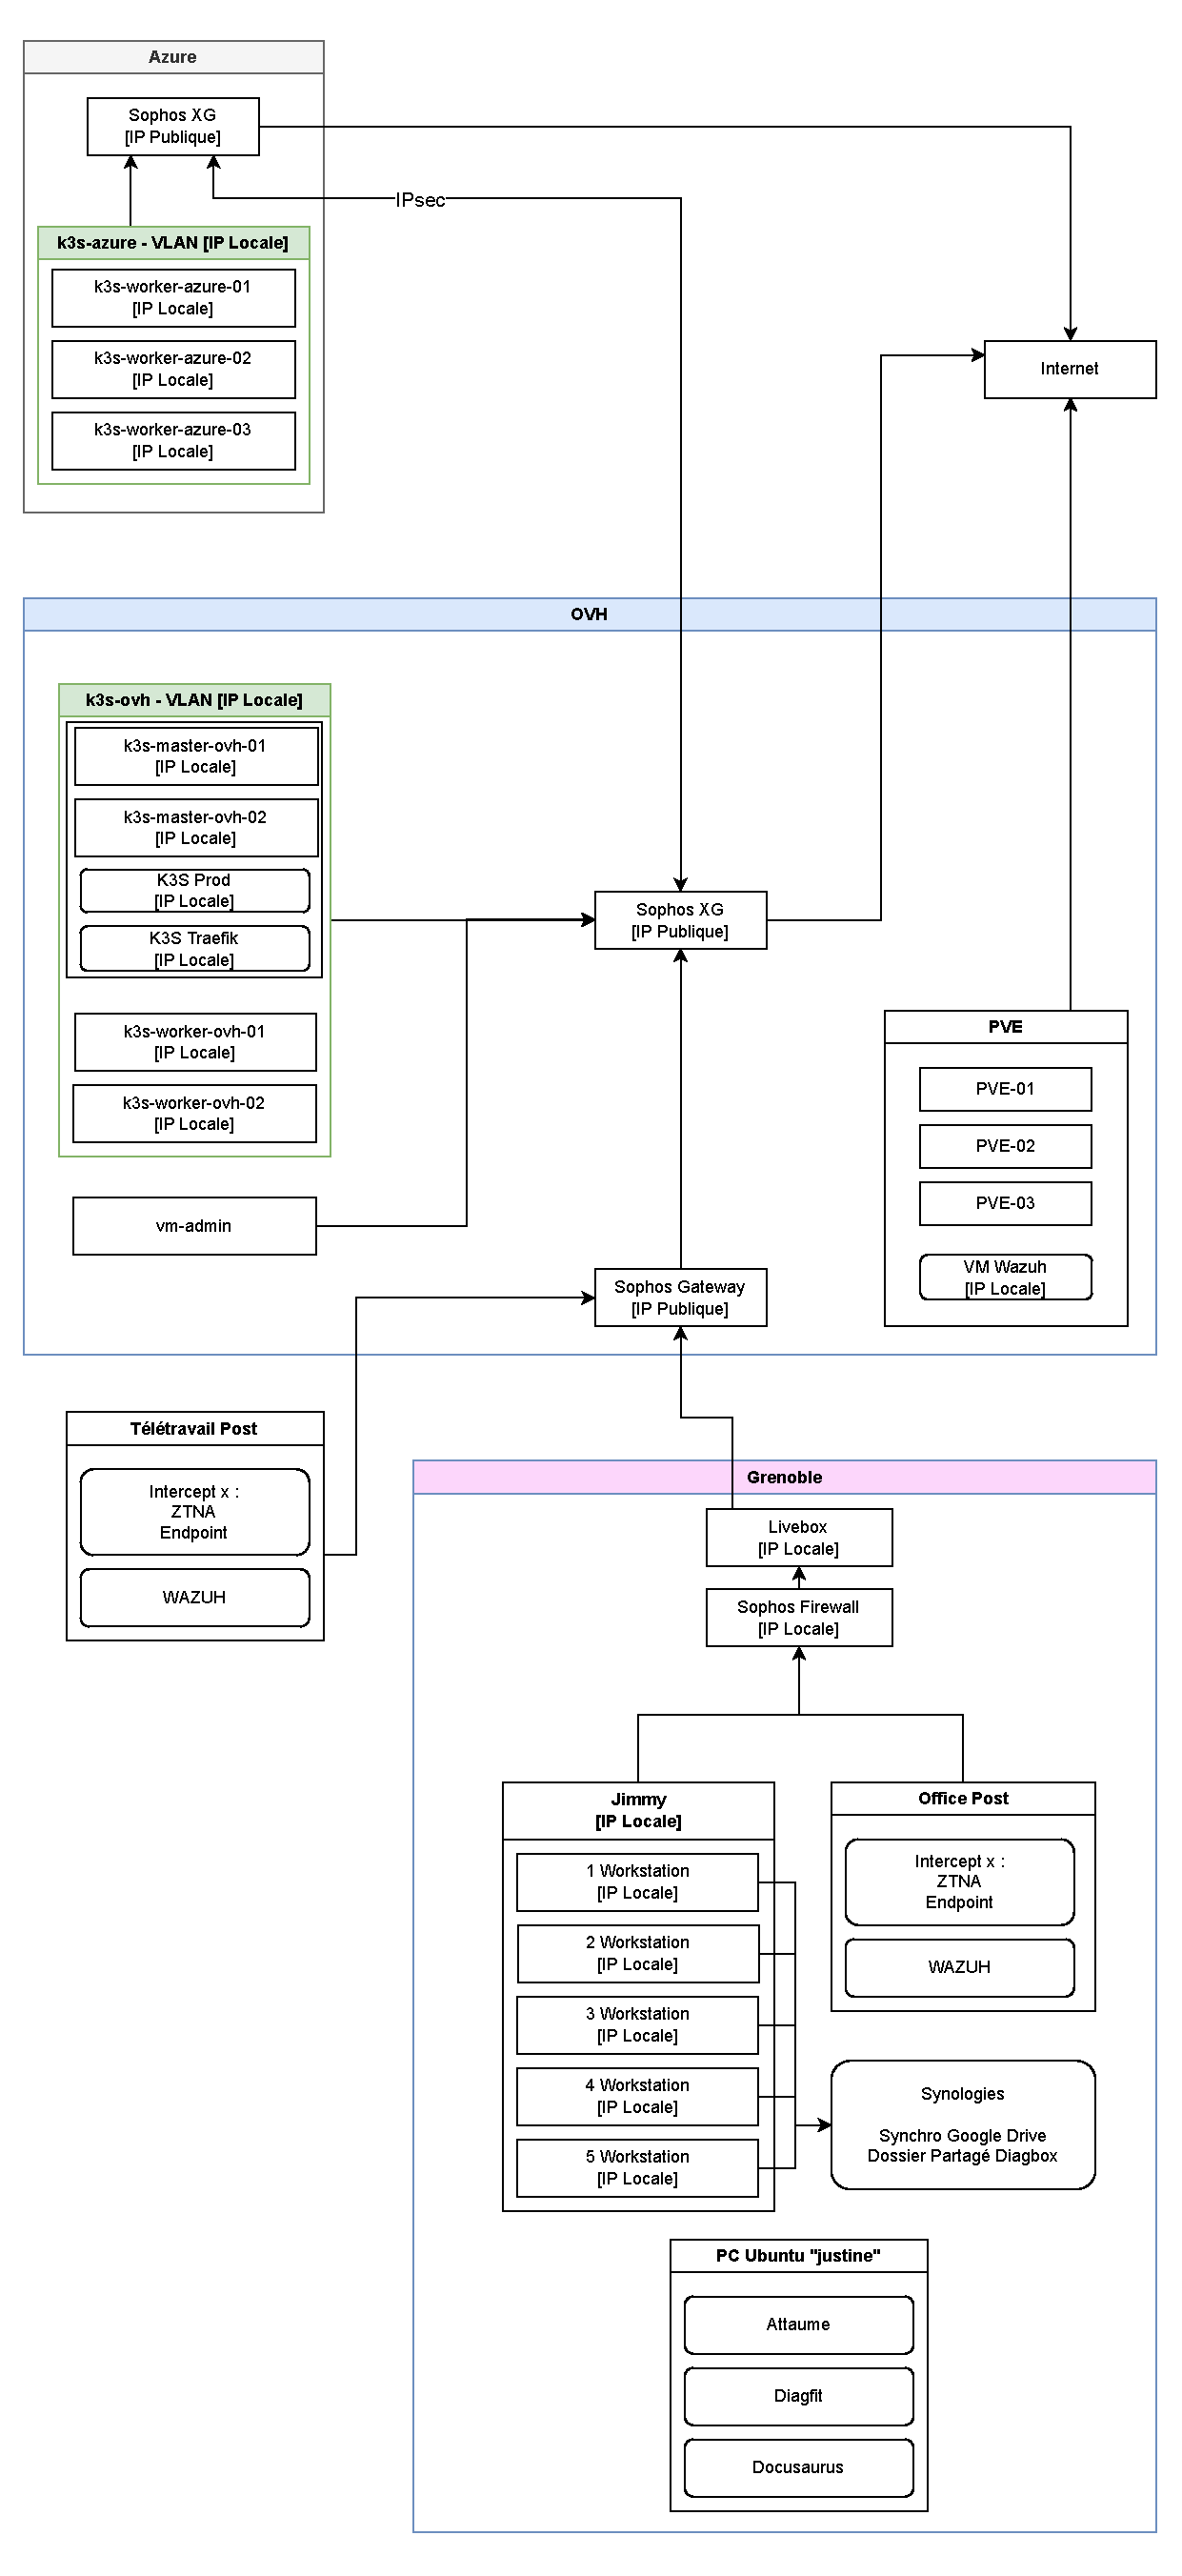
\includepdf{paper/figures/infra.pdf}
    \label{infra}
    \caption{Infrastructure}
\end{figure}
\restoregeometry % Rétablir la géométrie par défaut
\pagestyle{fancy}
\clearpage

\subsection*{Boucles de prise de décisions}
\begin{figure}[ht!]
    \centering
    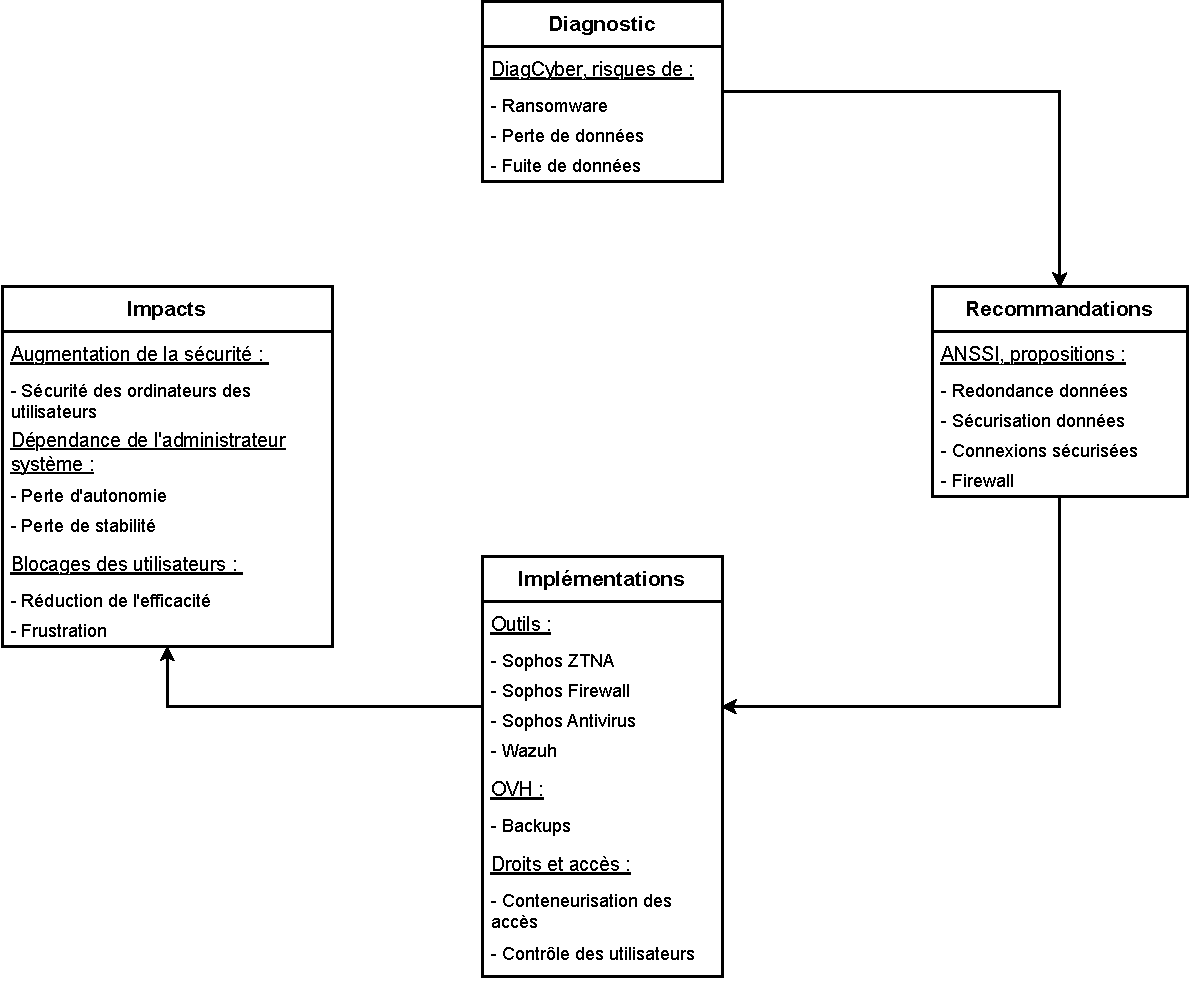
\includegraphics[width=0.5\textwidth]{paper/figures/boucle1.pdf}
    \caption{Première boucle du processus décisionnel}
    \label{fig:boucle1}
\end{figure}

\begin{figure}[ht!]
    \centering
    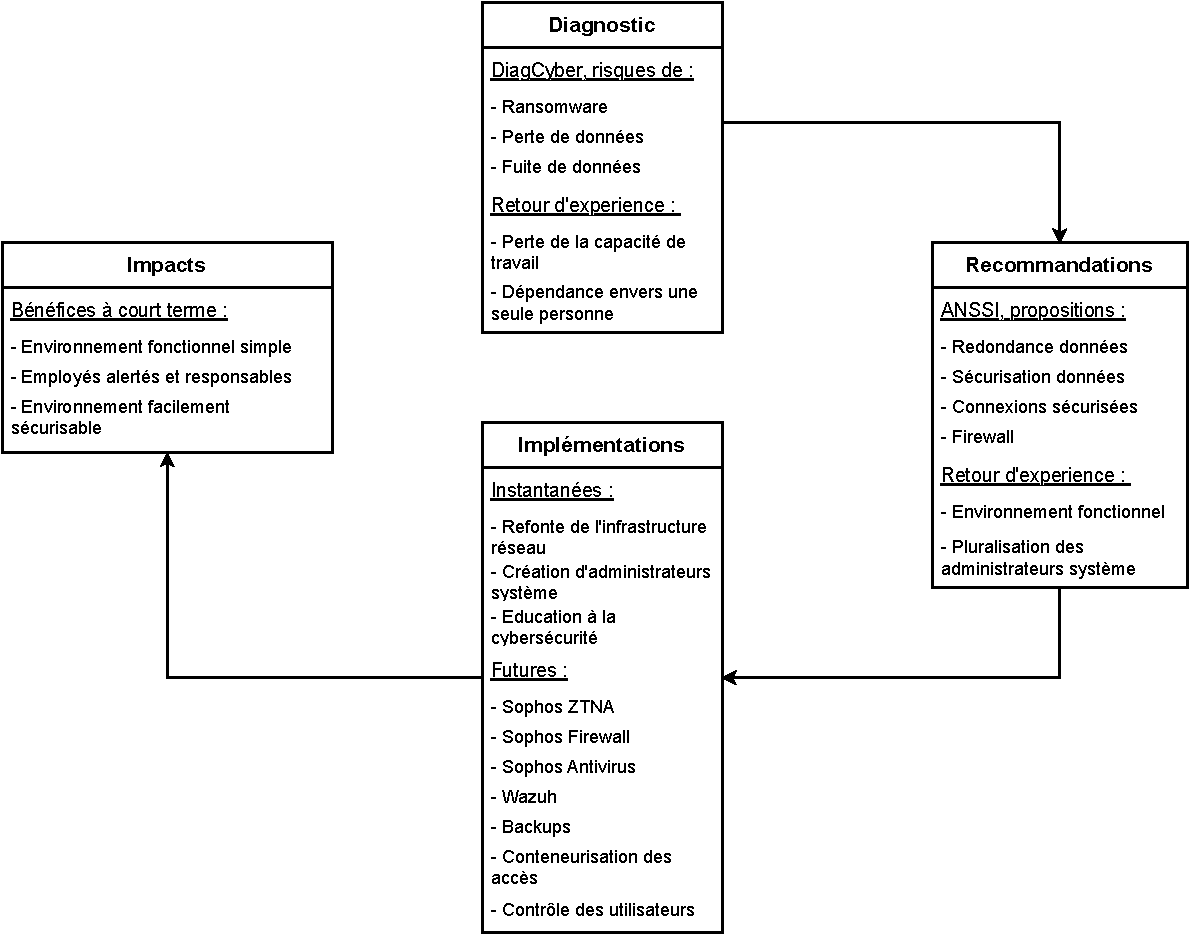
\includegraphics[width=0.5\textwidth]{paper/figures/boucle2.pdf}
    \caption{Seconde boucle du processus décisionnel}
    \label{fig:boucle2}
\end{figure}



\end{document}
